% Intestazione
\fancyhead[L]{3 \hspace{0.2cm} Architettura} % Testo a sinistra

\section{Architettura}
\label{sec:architettura}

Questa sezione fornisce una descrizione dettagliata dell'\emph{architettura logica}\textsubscript{\textbf{\textit{G}}} del prodotto software, illustrando le scelte progettuali adottate per garantire la corretta realizzazione del sistema. Saranno presentati le principali scelte e \emph{pattern architetturali}\textsubscript{\textbf{\textit{G}}}, e le \emph{componenti software}\textsubscript{\textbf{\textit{G}}} che compongono il sistema.

\subsection{Logica del Prodotto}
\label{sec:logica_prodotto}

\begin{figure}[h]
    \centering
    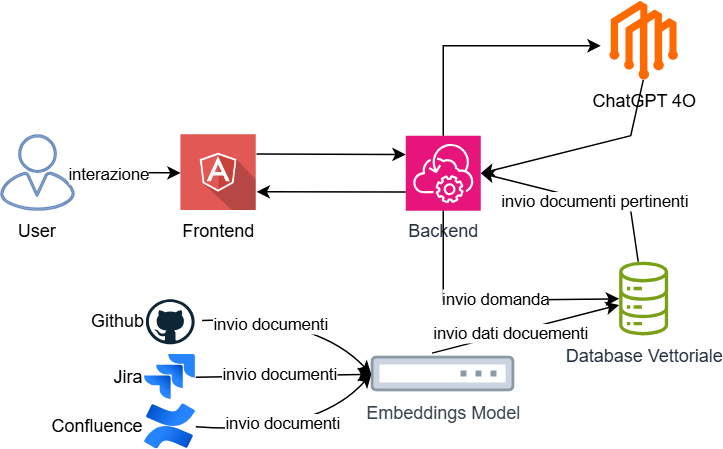
\includegraphics[width=\textwidth]{diagramma_specifica_tecnica.png}
    \caption{Logica del Prodotto}
\end{figure}

L’applicazione web permette di porre domande inerenti all’ecosistema aziendale
sfruttando un Large Language Model (LLM), nella fattispecie \emph{GPT-4o}\textsubscript{\textbf{\textit{G}}}, integrato con
un sistema di archiviazione e ricerca di documenti basato su tecniche di embedding
e su un database vettoriale.

L’applicazione permette agli utenti di ottenere risposte precise a domande relative all’ecosistema 
aziendale, utilizzando il Large Language Model \emph{GPT-4o}. La 
qualità delle risposte è garantita dall'integrazione diretta con documenti e dati provenienti dalle 
principali piattaforme interne (\emph{GithHub}\textsubscript{\textbf{\textit{G}}}, 
\emph{Jira}\textsubscript{\textbf{\textit{G}}} e \emph{Confluence}\textsubscript{\textbf{\textit{G}}}), 
sincronizzati automaticamente ogni 24 ore.
Tutti i documenti recuperati vengono suddivisi in parti più piccole e trasformati in vettori 
numerici attraverso un modello dedicato. Questi vettori, insieme ai relativi metadati, vengono 
archiviati stabilmente nel \emph{database vettoriale}\textsubscript{\textbf{\textit{G}}} 
\emph{chromaDB}\textsubscript{\textbf{\textit{G}}}, consentendo di effettuare rapidamente ricerche 
semantiche mirate.
Quando l’utente invia una domanda attraverso l’interfaccia web, il \emph{frontend}\textsubscript{\textbf{\textit{G}}} 
inoltra la richiesta al \emph{backend}\textsubscript{\textbf{\textit{G}}}. Quest’ultimo esegue una 
ricerca semantica all'interno del \emph{database vettoriale}\textsubscript{\textbf{\textit{G}}} per 
identificare le informazioni più rilevanti in relazione alla domanda posta. Il 
\emph{backend}\textsubscript{\textbf{\textit{G}}} invia quindi la domanda originale dell’utente, i 
risultati della ricerca semantica e un apposito \emph{prompt}\textsubscript{\textbf{\textit{G}}} al 
modello \emph{GPT-4o}. Tale \emph{prompt} 
fornisce istruzioni precise al modello, indicando il contesto aziendale di riferimento e definendo il 
formato desiderato della risposta.
\emph{GPT-4o} genera dunque una risposta contestualizzata, 
integrando automaticamente una sezione denominata \emph{“Link utili”} contenente tutti i riferimenti 
ai documenti aziendali utilizzati nella formulazione della risposta stessa. Qualora la domanda 
dell'utente risulti chiaramente fuori contesto aziendale, il chatbot risponderà con 
\emph{“domanda fuori contesto”}. Nel caso in cui non siano presenti documenti o informazioni pertinenti 
nel \emph{database vettoriale}, la risposta fornita sarà 
\emph{“nessuna informazione trovata”}.
Tutte le conversazioni tra utente e chatbot vengono salvate in modo persistente nel 
\emph{database PostgreSQL}\textsubscript{\textbf{\textit{G}}}. Al primo caricamento dell’applicazione, 
l'interfaccia mostra automaticamente gli ultimi cinquanta messaggi scambiati. Se l'utente desidera 
consultare messaggi precedenti, può scorrere verso l'alto e ulteriori messaggi vengono caricati 
progressivamente. Inoltre, dopo ciascuna risposta, il \emph{frontend} 
richiede al \emph{backend} di generare e suggerire domande di 
approfondimento, stimolando ulteriori interazioni coerenti con la conversazione in corso. L'interfaccia 
permette infine di copiare rapidamente le risposte del chatbot, comprese eventuali porzioni di codice 
presenti al loro interno.
Per quanto riguarda la gestione degli errori, l’applicazione notifica l’utente tramite messaggi 
dedicati qualora si riscontrassero problemi nel recupero di documenti o messaggi dal database
\emph{PostgreSQL} o durante la sincronizzazione con le 
piattaforme aziendali. Anche eventuali difficoltà nella generazione di risposte o nel caricamento delle 
domande suggerite vengono gestite informando tempestivamente l’utente e consentendo, ove possibile, di 
continuare ad utilizzare il servizio in modalità limitata o di riprovare successivamente.


\subsection{Architettura logica}
L’architettura adottata nella realizzazione dell’applicativo si basa sul modello di \emph{architettura esagonale}\textsubscript{\textbf{\textit{G}}}. Il livello di \emph{business}\textsubscript{\textbf{\textit{G}}} del software è quindi indipendente dagli altri componenti, ovvero nulla presente all’esterno della logica di business può conoscere la sua \emph{implementazione}\textsubscript{\textbf{\textit{G}}}. Questo principio alla base dell’architettura esagonale ci permette di ottenere un prodotto software facilmente testabile e \emph{manutenibile}\textsubscript{\textbf{\textit{G}}}. Le componenti che devono restare indipendenti sono rappresentate dal \emph{Domain business model}\textsubscript{\textbf{\textit{G}}}, che non comunica mai direttamente con l’esterno.
Gli elementi che permettono il funzionamento dell’architettura esagonale sono i seguenti:
\begin{itemize}
    \item \textbf{\emph{Controller}}\textsubscript{\textbf{\textit{G}}}: contiene l'\emph{application logic}\textsubscript{\textbf{\textit{G}}} del sistema: gestisce le richieste in ingresso, valida i dati di tipo \emph{DTO}\textsubscript{\textbf{\textit{G}}} ricevuti in input, e li adatta verso un tipo di dato di business. Il \emph{Controller} ha poi il compito di chiamare uno \emph{UseCase} per eseguire la logica di business, adattare l'output ricevuto in un oggetto DTO e restituirlo al client.
    \item \textbf{\emph{UseCase}}\textsubscript{\textbf{\textit{G}}}: rappresenta un caso d'uso specifico del sistema, che viene implementato da un \emph{Service} per realizzare la logica di business.
    \item \textbf{\emph{Service}}\textsubscript{\textbf{\textit{G}}}: contiene la \emph{business logic}\textsubscript{\textbf{\textit{G}}} del sistema: esegue operazioni specifiche esclusive del dominio di interesse e delega le interazioni con le altre componenti ai \emph{Port}. I \emph{Service} possono interagire unicamente con tipi di dato di business, garantendo l'indipendenza della logica di business dal resto del sistema.
    \item \textbf{\emph{Port}}\textsubscript{\textbf{\textit{G}}}: definisce le interfacce attraverso le quali i \emph{Service} interagiscono con il mondo esterno, permettendo il salvataggio e recupero di dati persistenti senza modificare la logica di business.
    \item \textbf{\emph{Adapter}}\textsubscript{\textbf{\textit{G}}}: implementa una o più interfacce definite dai \emph{Port}, permettendo la comunicazione tra la logica di business e le tecnologie esterne di \emph{persistent logic}\textsubscript{\textbf{\textit{G}}}. L'\emph{adapter} si occupa di adattare i dati ricevuti dalla logica di business in un tipo \emph{Entity}\textsubscript{\textbf{\textit{G}}} adatto per la persistenza, e viceversa.
    \item \textbf{\emph{Repository}}\textsubscript{\textbf{\textit{G}}}: contiene la \emph{persistent logic} del sistema: gestisce la persistenza dei dati, interagendo con un database o altre forme di storage per salvare e/o recuperare le informazioni necessarie. I tipi di dato gestiti dal \emph{repository} sono gli \emph{Entity}, che rappresentano il livello intermedio che sta a contatto diretto con i dati persistenti del sistema.
\end{itemize}

È stato scelto di utilizzare un'architettura esagonale per i seguenti motivi:
\begin{itemize}
    \item \textbf{Facilità di test}: l'architettura esagonale permette di testare facilmente la business logic, in quanto è possibile sostituire gli adapter con degli \emph{stub}\textsubscript{\textbf{\textit{G}}} o dei \emph{mock}\textsubscript{\textbf{\textit{G}}};
    \item \textbf{\emph{Manutenibilità}}\textsubscript{\textbf{\textit{G}}}: l'architettura esagonale permette di mantenere la business logic indipendente dagli altri componenti, facilitando la manutenzione del codice;
    \item \textbf{\emph{Scalabilità}}\textsubscript{\textbf{\textit{G}}}: l'architettura esagonale permette di aggiungere nuovi adapter senza dover modificare la business logic.
\end{itemize}


\subsection{Architettura di Deployment}
\label{sec:architettura_deployment}

Per determinare l'\emph{architettura di deployment}\textsubscript{\textbf{\textit{G}}} più adatta all'applicativo, si è tenuto conto del contesto reale in cui verrà utilizzato. Poiché il sistema è destinato all'utilizzo in un'azienda, dove non si prevedono significative espansioni o modifiche strutturali dopo l'installazione, la scelta di un'architettura monolitica è risultata la più appropriata. Questa soluzione, oltre a essere perfettamente in linea con le esigenze del prodotto, semplifica le fasi di progettazione, sviluppo e test. Inoltre, rispetto a un'architettura a microservizi, la monolitica evita complessità che sarebbero state difficili da gestire, anche considerando le competenze attuali del team di sviluppo.\\\\
Il deployment del prodotto viene gestito attraverso la containerizzazione con \textbf{\emph{Docker Compose}}\textsubscript{\textbf{\textit{G}}}. Questa scelta consente di semplificare l’installazione dell’applicativo, fornendo un ambiente preconfigurato in cui tutte le dipendenze sono già risolte. In questo modo, vengono predisposti automaticamente tutti i servizi necessari per garantire il corretto funzionamento del sistema, riducendo le difficoltà legate alla configurazione manuale.



\subsection{Architettura di dettaglio}
\label{sec:architettura_di_dettaglio}

\subsubsection{Architettura della generazione di una risposta}
\label{sec:architettura_generazione_risposta}

\begin{figure}[h]
    \centering
    
\includegraphics[width=\textwidth]{placeholder.png}
    \caption{Architettura della generazione di una risposta}
\end{figure}

L'\emph{UML}\textsubscript{\textbf{\textit{G}}} in questione rappresenta l'\emph{architettura}\textsubscript{\textbf{\textit{G}}} della generazione di una risposta all'interrogazione di un utente, dal punto di vista del \emph{backend}\textsubscript{\textbf{\textit{G}}}.
Il \emph{frontend}\textsubscript{\textbf{\textit{G}}} invoca il metodo \texttt{chat} esposto dal \emph{backend}\textsubscript{\textbf{\textit{G}}} tramite \emph{FastAPI}\textsubscript{\textbf{\textit{G}}}, passando la domanda dell'utente in forma di dizionario.
La domanda viene recuperata dal ChatController, che converte la stringa interna al dizionario in un oggetto di Business, Question, e lo invia all'interfaccia ChatUseCase, implementata da ChatService.
ChatService, che implementa il \emph{Design Pattern} \emph{Facade}\textsubscript{\textbf{\textit{G}}}, chiama SimilaritySearchService, componente responsabile della ricerca di \emph{similarità}\textsubscript{\textbf{\textit{G}}} nel \emph{database vettoriale}\textsubscript{\textbf{\textit{G}}}, il quale si collega con SimilaritySearchPort verso l'esterno, sfruttando l'\emph{architettura esagonale}\textsubscript{\textbf{\textit{G}}}. La Porta viene implementata da ChromaVectorStoreAdapter, che adatta la Question verso un tipo stringa inviato a ChromaVectorStoreRepository, che gestisce il collegamento con il database vettoriale \emph{Chroma}\textsubscript{\textbf{\textit{G}}}, sul quale avviene la ricerca di similarità. Una volta ottenuti i risultati della ricerca e trasformati in \emph{Entity}\textsubscript{\textbf{\textit{G}}}, essi vengono convertiti nel tipo di Business Document e poi restituiti a ChatService, il quale dunque li invia assieme all'input dell'utente a GenerateAnswerService, classe di servizio munita di un attributo Header che consente di fornire un introduzione di contesto al chatbot. Header, input utente e documenti rilevanti vengono quindi forniti a LangChainAdapter, che si assicura che la somma dei \emph{token}\textsubscript{\textbf{\textit{G}}} dei parametri non superi la soglia limite per l'\emph{LLM}\textsubscript{\textbf{\textit{G}}} configurato. Infine, i parametri vengono forniti a LangChainRepository, che li combina assieme in unico prompt e, sfruttando gli strumenti forniti dalla libreria \emph{LangChain}\textsubscript{\textbf{\textit{G}}}, effettua una chiamata verso l'LLM di \emph{OpenAI}\textsubscript{\textbf{\textit{G}}} configurato per ottenere una risposta. 
La risposta viene quindi convertita in un oggetto Answer di \emph{Business Logic}\textsubscript{\textbf{\textit{G}}} ed infine convertita in stringa per essere inserita in un dizionario in ChatController, il quale restituisce la risposta al frontend.

\newpage


\subsubsection{Architettura dell'aggiornamento automatico del database vettoriale}
\label{sec:architettura_aggiornamento_database_vettoriale}

\begin{figure}[h]
    \centering
    
\includegraphics[width=\textwidth]{placeholder.png}
    \caption{Architettura dell'aggiornamento automatico del database vettoriale}
\end{figure}

L'UML in questione rappresenta l'architettura dell'aggiornamento automatico del \emph{database vettoriale}\textsubscript{\textbf{\textit{G}}}, il quale viene svolto da un \emph{cron}\textsubscript{\textbf{\textit{G}}} configurato periodicamente per eseguire un apposito script \emph{Python}\textsubscript{\textbf{\textit{G}}}. Il cron chiama il metodo load della classe LoadFilesController, che a sua volta chiama l'interfaccia LoadFilesUseCase implementata da LoadFilesService.\\
LoadFilesService implementa il pattern \emph{Facade}\textsubscript{\textbf{\textit{G}}} per fornire un'unica interfaccia di collegamento alle piattaforme dalle quali caricare i file e alle piattaforme per il salvataggio degli stessi file e dei log di tutte le operazioni. In particolare, LoadFilesService si collega alle interfacce GitHubPort, JiraPort e ConfluencePort, che poi verranno implementate dai rispettivi adapter, che possiederanno i rispettivi repositories, rispettando l'\emph{Architettura Esagonale}\textsubscript{\textbf{\textit{G}}}. Vengono quindi recuperati i Commits e i Files da \emph{GitHub}\textsubscript{\textbf{\textit{G}}}, le Issues da \emph{Jira}\textsubscript{\textbf{\textit{G}}} e le pagine da \emph{Confluence}\textsubscript{\textbf{\textit{G}}}, estratti dagli account configurati, che vengono prima convertiti in oggetti \emph{Entity} nei repositories, e poi nel tipo di business Document mediante gli adapter. I documenti corrispondenti ai file di GitHub, una volta tornati a LoadFilesService, vengono confrontati con i commit GitHub per rilevare la loro data di creazione, mentre i documenti corrispondenti alle pagine di Confluence, una volta tornati a LoadFilesService, vengono "puliti" da tag ed entities HTML grazie all'attributo di tipo ConfluenceCleanerService di quest'ultima classe. La lista di oggetti Document viene dunque inviata a LoadFilesInVectorStorePort, implementata da ChromaVectorStoreAdapter, che si occupa di adattare i Document in DocumentEntity per poi inviarli a ChromaVectorStoreRepository, che si occupa di salvare i documenti nel database vettoriale \emph{Chroma}\textsubscript{\textbf{\textit{G}}}. Nel salvataggio, viene anche chiaramento distinto il numero di documenti aggiunti per la prima volta, il numero di documenti modificati ed il numero di documenti eliminati: viene considerata la data di ultimo aggiornamento per le Jira Issues, le Confluence Pages e i GitHub Commits, mentre avviene il confronto tra la data di creazione e la data di ultimo inserimento in Chroma per i GitHub Files. \\
Ogni classe di repository, oltre a svolgere il proprio di compito, si occupa anche di creare e restituire uno specifico oggetto di log, di tipo PlatformLog per GitHUb, Jira e Confluence e di tipo VectorStoreLog per il database vettoriale, che vengono uniti assieme in un oggetto LoadingAttempt e poi inviati all'interfaccia SaveLoadingAttemptInDbPort, implementata da PostgresAdapter, che si occupa di adattare l'oggetto in PostgresLoadingAttempt e di inviarlo a PostgresRepository che lo salva nel \emph{database relazionale}\textsubscript{\textbf{\textit{G}}} \emph{Postgres}\textsubscript{\textbf{\textit{G}}}, per tenere traccia dell'esito di ogni tentativo di caricamento di documenti nel database vettoriale. Successivamente, lo stesso log, opportunamente formattato, viene salvato in un file di testo, situato dentro la cartella \texttt{src/backend}.

\newpage


\subsubsection{Architettura del rendering dello storico, al caricamento iniziale e allo scroll}
\label{sec:architettura_rendering_storico}

\begin{figure}[h]
    \centering
    
\includegraphics[width=\textwidth]{placeholder.png}
    \caption{Architettura del rendering dello storico, al caricamento iniziale e allo scroll}
\end{figure}

L'UML in questione rappresenta l'architettura del rendering dello storico, al caricamento iniziale e allo scroll, cioè descrive tutte quelle operazioni compiute dai componenti e servizi di Angular per garantire che, all'avvio ed allo scroll verso il basso, sia visualizzabile una lista di messaggi, recuperati dal backend, nella schermata principale della pagina web.\\
Il componente ChatContainer, alla sua istanziazione, chiama il proprio metodo \texttt{loadOldMessages}, che chiama \texttt{getMessages} di DatabaseService passando come parametri la quantità di messaggi da ottenere e il numero della pagina da cui prelevarli. Una pagina raggruppa un certo numero di messaggi caricati in unico passaggio: nel caso del caricamento iniziale, la pagina da caricare è la pagina 1, cioè la pagina dei messaggi più recenti, mentre, nel caso dello scroll, viene chiamata la pagina successiva rispetto a quella che si sta visualizzando in quel momento. Il metodo \texttt{getMessages} di DatabaseService invoca dunque il metodo \texttt{get\_messages} esposto dal backend tramite FastAPI, passando come parametro un dizionario che indica la quantità di messaggi da ottenere e il numero di pagina, che lancia la catena descritta in \bulref{sec:architettura_recupero_messaggi_storico}. Una volta ottenuta la lista di oggetti serializzati dal backend, DatabaseService si occupa di creare una lista di oggetti di tipo Message, che restituisce a ChatContainer. ChatContainer, poi, si occupa di formattare appositamente, tra la lista dei messaggi, i messaggi scritti dal chatbot, per evidenziare parole e zone di interesse delle risposte.\\
Poi, nel caso in cui si sia in fase di caricamento iniziale, ChatContainer chiama il proprio metodo scrollToBottom, che chiama il metodo scrollToBottom di ChatMessages, che fa in modo che l'utente visualizzi nella schermata iniziale i messaggi più recenti. Altrimenti, nel caso di scroll verso il basso, e quindi di caricamento di messaggi sovrastanti quelli già presenti, è necessario ricalibrare la barra di scorrimento laterale senza che cambi la schermata visualizzata dall'utente, e dunque ChatContainer chiama l'apposita funzione maintainScrollPosition di ChatMessages.

\newpage


\subsubsection{Architettura del rendering grafico di domanda e risposta}
\label{sec:architettura_rendering_domanda_risposta}

\begin{figure}[h]
    \centering
    
\includegraphics[width=\textwidth]{placeholder.png}
    \caption{Architettura del rendering grafico di domanda e risposta}
\end{figure}

L'UML in questione rappresenta l'architettura del rendering grafico di domanda e risposta, cioè descrive tutte quelle operazioni compiute dai componenti e servizi di Angular durante l'interazione tra utente e chatbot per renderizzare visivamente la chat.\\
ChatInput, il componente che contiene la barra di input e il pulsante di invio, all'evento di invio di una domanda da parte dell'utente risponde con il metodo \texttt{onSend}, il quale chiama \texttt{onSendMessage} di ChatContainer, che inizialmente crea un oggetto Message e lo stampa visivamente a schermo, per poi chiamare \texttt{scrollToBottom} per scorrere in basso. Poi, ChatContainer si occupa di far partire il salvataggio del messaggio chiamando il metodo \texttt{saveMessage} di DatabaseService, che a sua volta chiama il metodo \texttt{save\_message} esposto dal backend tramite FastAPI, che segue la catena di classi descritta in \bulref{sec:architettura_salvataggio_messaggi_storico} fino a salvare il messaggio nel database relazionale Postgres. La risposta restituita per il salvataggio giunge dunque a ChatContainer e viene stampata sulla console. ChatContainer chiama allora il metodo \texttt{sendMessage} di ChatService, che a sua volta chiama \texttt{get\_answer} esposto da FastAPI che fa partire la catena descritta in \bulref{sec:architettura_generazione_risposta}. Una volta ottenuto il dizionario di stringhe come risposta, \dots

\newpage


\subsubsection{Architettura frontend dell’aggiornamento del badge di segnalazione dell’esito dell’ultimo aggiornamento automatico}
\label{sec:architettura_frontend_badge_aggiornamento}

\begin{figure}[h]
    \centering
    
\includegraphics[width=\textwidth]{placeholder.png}
    \caption{Architettura frontend dell’aggiornamento del badge di segnalazione dell’esito dell’ultimo aggiornamento automatico}
\end{figure}

\dots

\newpage


\subsubsection{Architettura backend dell’aggiornamento del badge di segnalazione dell’esito dell’ultimo aggiornamento automatico}
\label{sec:architettura_backend_badge_aggiornamento}

\begin{figure}[h]
    \centering
    
\includegraphics[width=\textwidth]{placeholder.png}
    \caption{Architettura backend dell’aggiornamento del badge di segnalazione dell’esito dell’ultimo aggiornamento automatico}
\end{figure}

L'UML in figura rappresenta l'architettura dell'aggiornamento del badge di segnalazione dell'esito dell'ultimo aggiornamento automatico, dal punto di vista del backend. Il frontend invoca il metodo\\ \texttt{get\_last\_load\_outcome} esposto dal backend tramite FastAPI, il quale chiama GetLastLoadOutcomeController, che a sua volta chiama l'interfaccia GetLastLoadOutcomeUseCase implementata da GetLastLoadOutcomeService. GetLastLoadOutcomeService chiama l'interfaccia GetLastLoadOutcomePort, implementata da PostgresAdapter, che invoca il metodo \texttt{get\_last\_load\_outcome} esposto da PostgresRepository, che si occupa di recuperare da Postgres l'ultimo esito del caricamento di documenti nel database vettoriale Chroma. Più precisamente, viene recuperato l'attributo \texttt{outcome} della tupla con timestamp di fine aggiornamento più recente dalla tabella \texttt{loading\_attempts}. PostgresRepository restituisce un oggetto di tipo PostgresLastLoadOutcome, che può assumere valore True, se l'ultimo tentativo di aggiornamento ha avuto esito positivo, False, se l'ultimo tentativo di aggiornamento ha avuto esito negativo, o Error, se c'è stato un errore nell'interazione con Postgres per recuperare l'esito dell'ultimo aggiornamento. L'oggetto PostgresLastLoadOutcome viene convertito in un oggetto di tipo LastLoadOutcome da PostgresAdapter e restituito a GetLastLoadOutcomeService. Infine, GetLastLoadOutcomeController converte l'oggetto verso il tipo LastLoadOutcomeDTO e lo restituisce al frontend.

\newpage


\subsubsection{Architettura del salvataggio dei messaggi nello storico}
\label{sec:architettura_salvataggio_messaggi_storico}

\begin{figure}[h]
    \centering
    
\includegraphics[width=\textwidth]{placeholder.png}
    \caption{Architettura del salvataggio dei messaggi nello storico}
\end{figure}

L'\emph{UML} in figura rappresenta l'\emph{architettura} del salvataggio dei messaggi nello storico.
Il \emph{frontend} invoca il metodo \texttt{save\_message} esposto dal \emph{backend} tramite \emph{FastAPI}, passando il messaggio in forma di MessageDTO.
Il messaggio viene recuperato dal SaveMessageController, che converte il messaggio in un oggetto di Business, Message, e lo invia all'\emph{interfaccia}\textsubscript{\textbf{\textit{G}}} SaveMessageUseCase, implementata da SaveMessageService.
SaveMessageService, quindi, chiama l'interfaccia SaveMessagePort, che è implementata da PostgresAdapter.
PostgresAdapter si occupa di convertire il tipo di dato Message nel tipo PostgresMessage, e invoca il metodo \texttt{save\_message} esposto dalla classe PostgresRepository.
PostgresRepository gestisce il collegamento con il \emph{database relazionale}\textsubscript{\textbf{\textit{G}}} \emph{Postgres}\textsubscript{\textbf{\textit{G}}},
esegue l'operazione di salvataggio del messaggio sul database e restituisce un oggetto di tipo PostgresSaveOperationResponse che indica il successo o fallimento dell'operazione di salvataggio e la descrizione del successo o dell'eventuale errore.
Successivamente PostgresAdapter si occupa anche di convertire l'oggetto PostgresSaveOperationResponse in un DbSaveOperationResponse corrispondente e lo restituisce a SaveMessageService.
Infine SaveMessageController riceve la DbSaveOperationResponse e la converte in un dizionario da restituire a frontend, che gestirà appositamente il successo o l'errore.

\newpage


\subsubsection{Architettura del recupero dei messaggi dallo storico}
\label{sec:architettura_recupero_messaggi_storico}

\begin{figure}[h]
    \centering
    
\includegraphics[width=\textwidth]{placeholder.png}
    \caption{Architettura del recupero dei messaggi dallo storico}
\end{figure}

L'UML in figura rappresenta l'architettura del recupero dei messaggi nello storico.
Il frontend invoca il metodo \texttt{get\_messages} esposto dal backend tramite FastAPI, passando come parametro un dizionario che indica la quantità di messaggi da ottenere.
Il metodo \texttt{get\_messages} chiama GetMessagesController, che converte il dizionario in un oggetto Quantity e lo passa all'interfaccia GetMessagesUseCase, implementata da GetMessagesService.
GetMessagesService, quindi, chiama l'interfaccia GetMessagesPort, che è implementata da PostgresAdapter.
PostgresAdapter converte l'oggetto Quantity in un intero da passare come parametro alla classe PostgresRepository, che gestisce il collegamento con il database relazionale Postgres. 
PostgresRepository esegue l’operazione di recupero della quantità di messaggi richiesti e restituisce una lista di messaggi di tipo PostgresMessage.
Allora PostgresAdapter si occupa di convertirla in una lista di oggetti Message, che viene restituita all'indietro a GetMessagesService.
Infine GetMessagesController riceve una lista di Message e la usa per creare una lista di MessageDTO che restituisce al frontend.

\newpage


\subsubsection{Architettura della generazione di domande per proseguire la conversazione}
\label{sec:architettura_generazione_domande_conversazione}

\begin{figure}[h]
    \centering
    
\includegraphics[width=\textwidth]{placeholder.png}
    \caption{Architettura della generazione di domande per proseguire la conversazione}
\end{figure}

L'UML in figura rappresenta l'architettura della generazione di domande per proseguire la conversazione.
Il frontend invoca il metodo \texttt{get\_next\_possible\_questions} esposto dal backend tramite FastAPI, passando come parametro un dizionario che contiene l'ultima domanda dell'utente, l'ultima risposta del chatbot e la quantità di domande da ottenere.
Il metodo \texttt{get\_next\_possible\_questions} chiama GetNextPossibleQuestionsController, che converte il dizionario in un oggetto QuestionAnswerCouple contenente domanda (di tipo Question) e risposta (di tipo Answer) e in un oggetto Quantity contenente la quantità richiesta, e lo passa all'interfaccia GetNextPossibleQuestionsUseCase, implementata da GetNextPossibleQuestionsService.
GetNextPossibleQuestionsService possiede un attributo di tipo Header contenente un'introduzione di contesto per l'\emph{LLM}\textsubscript{\textbf{\textit{G}}}, templatizzata sulla base del numero di domande da richiedere, che a questo punto viene stabilito in base al parametro Quantity. L'attributo di tipo Header contiene anche importanti istruzioni di sintassi che l'\emph{LLM} deve rispettare, cioè impone che le possibili domande generate sia l'unico contenuto del messaggio e siano separate da \_\_. La classe GetNextPossibleQuestionsService chiama dunque l'interfaccia GetNextPossibleQuestionsPort con parametri QuestionAnswerCouple ed Header.
L'interfaccia è implementata da LangChainAdapter, che si occupa di adattare i parametri da QuestionAnswerCouple ed Header a due tipi stringa, per poi inviarli a LangChainRepository, che si occupa di invocare l'\emph{LLM} configurato per ottenere le possibili domande successive, in forma di un'unica stringa. Quest'ultima nell'Adapter viene suddivisa in 3 oggetti PossibleQuestion, sfruttando il fatto che l'header ha imposto all'LLM che le domande siano separate da \_\_, e, insieme ad un intero num\_questions che indica il numero di domande, vengono poi riunite in un oggetto NextPossibleQuestions, per essere quindi restituite a GetNextPossibleQuestionsService.
Infine GetNextPossibleQuestionsController riceve l'oggetto NextPossibleQuestions, converte le domande contenute in un dizionario di stringhe, e lo restituisce al frontend.

\newpage



\subsection{Design pattern utilizzati}
\label{sec:design_pattern_utilizzati}


\subsubsection{Facade}
\label{sec:facade}

Il pattern \emph{Facade}\textsubscript{\textbf{\textit{G}}} è stato adottato per permettere al \emph{cron}\textsubscript{\textbf{\textit{G}}} di accedere ad unica classe LoadFilesService avente il compito di caricare tutti i tipi di file necessari per l'aggiornamento del database vettoriale. Questo pattern permette di nascondere la complessità del sistema, fornendo un'interfaccia semplificata per l'accesso alle funzionalità offerte dalla classe LoadFilesService. In questo modo, il cron non deve preoccuparsi di come i file vengono caricati, ma può semplicemente chiamare il metodo \texttt{load} della suddetta classe per ottenere il risultato desiderato.
E' stato inoltre adottato un piccolo Facade anche per l'architettura di generazione di una risposta, dove ChatService si occupa di nascondere la complessità della logica di business, fornendo un'interfaccia semplificata per l'accesso alle funzionalità offerte da SimilaritySearchService e GenerateAnswerService.
Grazie a questo pattern, è possibile mantenere il codice più pulito e manutenibile, in quanto la complessità è nascosta all'esterno e le interazioni con le classi interne sono semplificate.


\subsubsection{Dependency Injection}
\label{sec:dependency_injection}

Il pattern \emph{Dependency Injection}\textsubscript{\textbf{\textit{G}}} è stato adottato per permettere l'iniezione delle dipendenze all'interno delle classi del sistema. Questo pattern permette di separare la creazione degli oggetti dal loro utilizzo, semplificando la gestione delle dipendenze e rendendo il codice più manutenibile e testabile. In questo modo, le classi non devono preoccuparsi di come vengono creati gli oggetti di cui hanno bisogno, ma possono semplicemente riceverli come parametri di costruzione. Questo permette di sostituire facilmente le implementazioni delle dipendenze, senza dover modificare il codice di tutte le classi che le utilizzano. Inoltre, grazie all'utilizzo di un \emph{framework}\textsubscript{\textbf{\textit{G}}} di \emph{Dependency Injection}, come \emph{Angular}\textsubscript{\textbf{\textit{G}}}, è possibile automatizzare il processo di creazione e iniezione delle dipendenze, semplificando ulteriormente lo sviluppo del \emph{frontend}\textsubscript{\textbf{\textit{G}}}. Il pattern è stato implementato anche in \emph{Python}\textsubscript{\textbf{\textit{G}}} nel \emph{backend}\textsubscript{\textbf{\textit{G}}}, attraverso due funzioni, \texttt{dependency\_injection\_frontend} e \texttt{dependenc\_injection\_cron}, che si occupano di iniettare le dipendenze rispettivamente nel file di endpoint \emph{FastAPI}\textsubscript{\textbf{\textit{G}}} a cui accede il frontend per contattare il backend e nel file che viene eseguito periodicamente dal cron per l'aggiornamento del \emph{database vettoriale}\textsubscript{\textbf{\textit{G}}}.


\subsubsection{MVVM}
\label{sec:mvvm}

Il pattern \emph{MVVM}\textsubscript{\textbf{\textit{G}}} è stato adottato per la progettazione dell'architettura del \emph{frontend}, in particolare per separare la logica di presentazione dalla logica di business, semplificando la gestione delle interazioni tra i componenti dell'applicazione. Nello specifico, il \emph{Model}\textsubscript{\textbf{\textit{G}}} rappresenta i dati e la logica di business dell'applicazione, il \emph{View}\textsubscript{\textbf{\textit{G}}} si occupa della presentazione dei dati all'utente, e il \emph{ViewModel}\textsubscript{\textbf{\textit{G}}} si occupa di gestire la logica di presentazione e di coordinare le interazioni tra il \emph{Model} e la \emph{View}. Questo permette di mantenere il codice più pulito e manutenibile, in quanto la logica di business è separata dalla logica di presentazione, e le interazioni tra i componenti sono semplificate. Inoltre, grazie all'utilizzo di un \emph{framework} come \emph{Angular}, è possibile automatizzare il processo di creazione e gestione dei componenti, semplificando ulteriormente lo sviluppo del \emph{frontend}. Il pattern è stato implementato in \emph{Angular} attraverso la creazione di componenti per la \emph{View} e il \emph{ViewModel}, e la creazione di servizi per la gestione della logica di business del \emph{Model}.
